\chapter{Результаты}

\section{Сравнение методов первого и второго порядка}
\subsection{Решение уравнения в одном направлении}
Сравнение методов проводилось на следующей задаче. Рассматривалась
геометрическая область, куб со стороной $a = 2$. В центре области находится
крест, состоящий из пяти одинаковых кубиков со стороной $b = 0.2$ (см. рис. \ref{fig:6}).
\begin{figure}[ht!]
\centering{
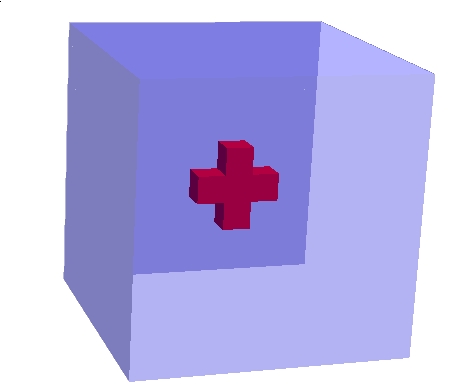
\includegraphics[width = 0.5\textwidth]{cross.png}
}
\caption{Расчетная область}
\label{fig:6}
\end{figure}
Коэффи\-циент поглощения в области равен $\varkappa_1=0$, а внутри креста - $\varkappa_2 = 100$. Равновесная интенсивность в центральной области $1$, а в окружающей среде - $0$. Решение строилось вдоль одного направления, $\omega = (0,0,1)$ на сетке с $415625$ тетраэдрами и $76247$ вершинами. Изучалось решение на выходящей грани куба. 
\begin{figure}[ht!]
\centering{
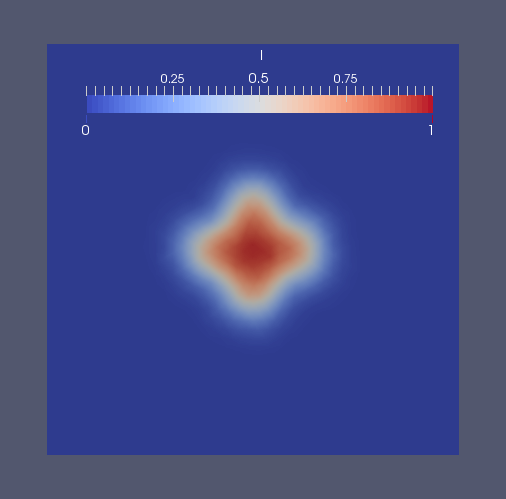
\includegraphics[width = 0.3\textwidth]{1ord.png}%
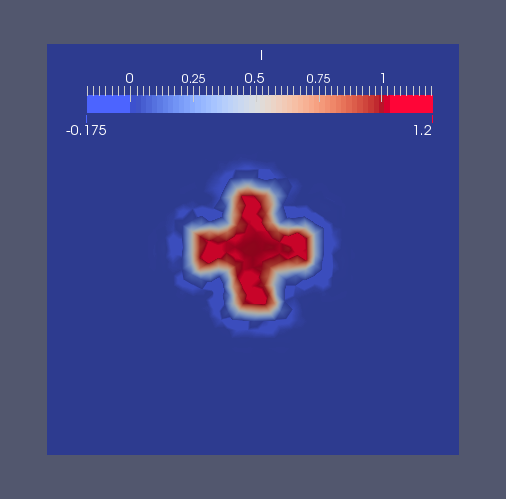
\includegraphics[width = 0.3\textwidth]{2nolim.png}%
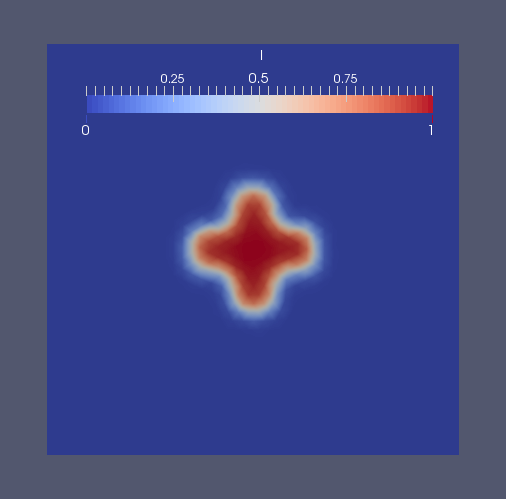
\includegraphics[width = 0.3\textwidth]{2wilim.png}
}
\caption{Сравнение решений методами первого порядка (слева), второго (в центре) и второго с ограничителем(справа).}
\label{fig:7}
\end{figure}

Точное решение должно представлять собой крест с интенсивностью $1 -
e^{b\varkappa_2} = 1-e^{-20} \approx 1$. Мы можем видеть (см. рис. \ref{fig:7}), что для первого порядка диффузия достаточно велика, второй порядок без ограничителя отклоняется от допустимых пределов $I \in [0, 1]$ на $20 \%$.
\subsection{Сравнение плотности излучения}
На той же самой задаче изучалась плотность излучения в центральном сечении куба, но коэффициенты поглощения изменились следующим образом: $\varkappa_1 = 10$, $\varkappa_2 = 1$. . Использовались 170 направлений из квадратурной формулы Лебедева \cite{lebedev_1999}. 

\begin{figure}[ht!]
\centering{
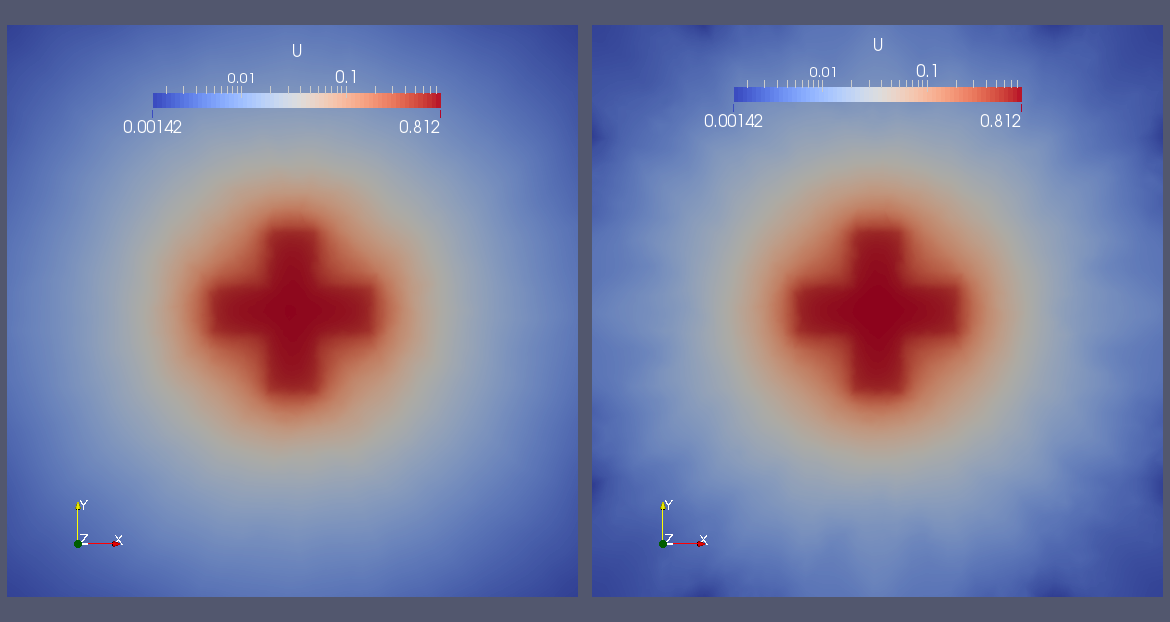
\includegraphics[width = \textwidth]{U2vs1.png}
}
\caption{Сравнение плотности излучения в центральном сечении куба. Слева второй порядок, справа --- первый.}
\label{fig:9}
\end{figure}

\begin{figure}[ht!]
\centering{
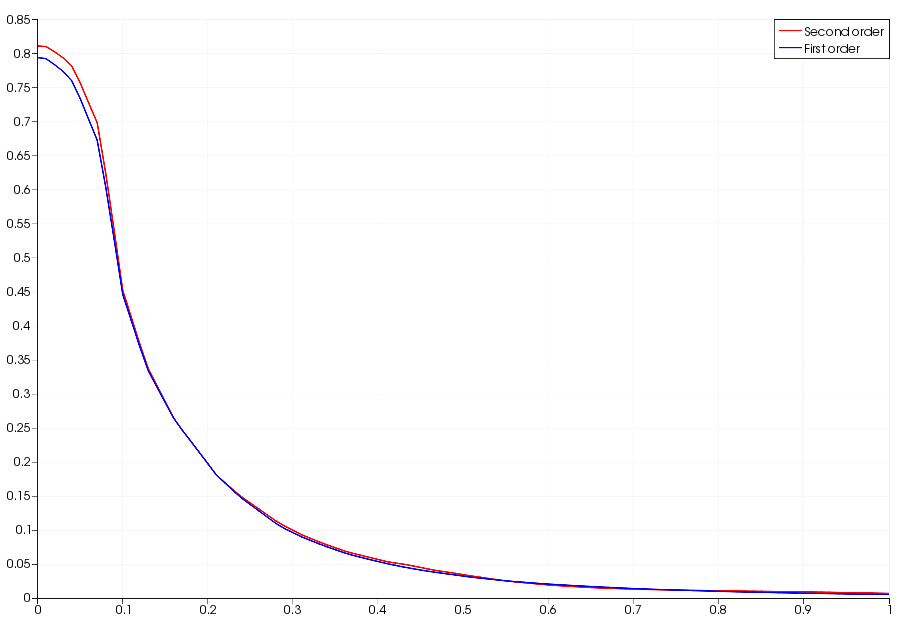
\includegraphics[width = \textwidth]{U2vs1Line.png}
}
\caption{Плотность излучения вдоль оси $Oz$. Красный второй порядок, синий - первый.}
\label{fig:10}
\end{figure}
Сравнение плотности излучения \ref{fig:9} и \ref{fig:10} показывает схожие результаты: интенсивность в центре куба в методе второго порядка на $\approx 2 \%$ больше, чем в случае метода первого порядка. В случае метода второго порядка \ref{fig:9} более выражен <<эффект луча>>, в то время как в методе первого порядка этот эффект сглажен за счет численной диффузии. 

\section{Сравнение методов первого и второго порядка с одинаковым количеством степеней свобод}
\section{Более сложная задача из астрофизики}
